\documentclass[bibtex,bwlinks,openright,twoside,fullbib,a4paper,english]{styles/thesis}

\usepackage{ifpdf}
\usepackage{ifthen}

\ifthenelse{\boolean{pdf}}
{
\usepackage[pdftex]{graphicx}
}{
\usepackage[dvips]{graphicx}
}

	
\usepackage{amsmath}
\usepackage{mathpple}
%% \usepackage{palatino}
\usepackage[LGR,T1]{fontenc}
\def\sfdefault{cmss}

\usepackage{tabularx}
\usepackage{calc}
\usepackage{comma}
\usepackage{listings}
\usepackage{lscape}

\usepackage[all]{xy}

\usepackage{thumbpdf}
\usepackage{enumerate}
\usepackage{dsfont}
\makeatletter
\let\comma\@commaform
\makeatother


\usepackage[bf,debug]{caption2}[2002/08/03]
%Definition of caption style
\newcaptionstyle{rmHang}{%
  \normalcaptionparams
  \renewcommand\captionlabelfont{\bfseries}%
  \renewcommand\captionlabeldelim{.}%
  \renewcommand\captionsize{\footnotesize}%
  \onelinecaptionsfalse
  \usecaptionstyle{hang}}
\newcaptionstyle{rmCenter}{%
  \normalcaptionparams
  \renewcommand\captionlabelfont{\bfseries}%
  \renewcommand\captionlabeldelim{.}%
  \renewcommand\captionsize{\footnotesize}%
  \onelinecaptionsfalse
  \usecaptionstyle{center}}
\newcaptionstyle{sfHang}{%
  \normalcaptionparams
  \renewcommand\captionlabelfont{\bfseries\sffamily}%
  \renewcommand\captionlabeldelim{.}%
  \renewcommand\captionfont{\sffamily}%
  \renewcommand\captionsize{\footnotesize}%
  \onelinecaptionsfalse
  \usecaptionstyle{hang}}
\newcaptionstyle{sfCenter}{%
  \normalcaptionparams
  \renewcommand\captionlabelfont{\bfseries\sffamily}%
  \renewcommand\captionlabeldelim{.}%
  \renewcommand\captionfont{\sffamily}%
  \renewcommand\captionsize{\footnotesize}%
  \onelinecaptionsfalse
  \usecaptionstyle{center}}
% Caption command shortcut
%\newcommand{\hcaption}[1]{\captionstyle{rmHang}\caption{#1}}
%\newcommand{\ccaption}[1]{\captionstyle{rmCenter}\caption{#1}}
\newcommand{\hcaption}[2][nullnullnull]{\captionstyle{rmHang}\ifthenelse{\equal{#1}{nullnullnull}}{\caption{#2}}{\caption[#1]{#2}}}
\newcommand{\ccaption}[2][nullnullnull]{\captionstyle{rmCenter}\ifthenelse{\equal{#1}{nullnullnull}}{\caption{#2}}{\caption[#1]{#2}}}
\allowdisplaybreaks


\lstset{frame=tb,
  language=C,
  aboveskip=1mm,
  belowskip=1mm,
  showstringspaces=false,
  columns=flexible,
  basicstyle={\small\ttfamily},
  numbers=none,
  keywordstyle=\color{blue},
  commentstyle=\color[rgb]{0.0,0.4,0.0},
  breaklines=true,
  breakatwhitespace=true,
  tabsize=4,
  emph={%  
    int32_t, float32%
    },emphstyle={\color{blue}}%
}

\begin{document}

\selectlanguage{english}

\author{Ghitti Marco}
\title{Title}{
\anno{2019/2020}
\matricola{893986}
\relatore{Prof.}
\ifthenelse{\boolean{pdf}}
{
\universita[./figures/poli.pdf]{Politecnico di Milano}%
}{
\universita[./figures/poli.eps]{Politecnico di Milano}%
}
{Facolt� di Ingegneria dell'Informazione}%
{Corso di laurea in Ingegneria Informatica}



%%% create front page %%%
\frontmatter
% acknowledgments go here
\thispagestyle{empty} \normalfont \cleardoublepage
\thispagestyle{empty}  \cleardoublepage
\pagenumbering{Roman}
\pagestyle{plain}

\chapter*{Abstract}
\addcontentsline{toc}{chapter}{Abstract}
Abstract content

\newpage

\chapter*{Ringraziamenti}
\addcontentsline{toc}{chapter}{Ringraziamenti}
Ringraziamenti


\mainmatter

\chapter{Introduction}
Intro content

\chapter{Definitions}
Intro

\section{Conclusions}

\chapter{State of the art}
In this chapter we explore previously existing implementations of developement stacks used to produce stream computing applications and deep learning accelerators. 

\newpage
\section{Chapter structure}
Section \ref{streamit} introduce StreamIt, a research compilation infrastructure to deploy optimized streaming applications from a high level definition.
Section \ref{vitis} describe VitisAI, a proprietary end-to-end developement stack to deploy DL models on Xilinx HW.
Section \ref{halide} describe Halide, a open source language and compilation infrastructure to produce optimized code for image and tensor processing.


\section{StreamIt}
\label{streamit}

Writing a program in the context of a streaming application while satisfying a set of requirements in terms of throughput and latency require a careful management of memory transfer and HW resources. That problem can be solved by writing custom code that directly manage these aspects but the development process is error prone and slow.

StreamIt is a programming language and research compilation infrastructure for streaming systems. It is an MIT project started in the year 2000 with the goal of executing high-performance streaming applications while increasing the programmer productivity through stream-specific abstractions. The compilation infrastructure take as input a program written with the StreamIt programming language, perform stream specific optimizations and produce the optimized final program to be deployed on the target architecture.

\newpage

\subsection{Streaming Application Domain}
The application domain of a streaming program is characterized by a set of assumptions that can be leveraged by a developement stack. By leveraging these characteristics a streaming programming language can increase performances while providing a set of abstractions that make easier for the programmer to write and maintain the source code of the application.

\subsubsection{Large stream of data}
The execution model of a general program is fundamentally different than the model of a streaming application: A common program is usually invoked with a finite input set that is kept until termination; instead, in the context of a streaming application the input is virtually infinite and is a sequence of data items where each element require a finite amount of operations before being discarded. A stream program can run indefinitely, waiting for items to be processed from an external input source.

\subsubsection{Independent stream filters}
To exploit the parallelism of a streaming application the programmer must specify a set of interconnected filters. The whole set of interconnected filters is referred as Stream Graph and contain information about communication among filters and how to exploit the intrinsic parallelism of the specific application.

Each filter define a self contained transformation on data items that can be executed independently from all others, while the connections among filters define the computation pattern, and thus the kind of parallelism that can be exploited.

\subsubsection{Stable computation pattern}
To be able to exploit the parallelism among filters and all other advantages of the streaming domain, the stream graph is assumed to be constant during steady state execution. The domain allow occasional modifications to the computation pattern but can lead to a significant performance degradation if used improperly by changing it's structure frequently.

\subsubsection{Occasional out-of-stream communication}
Even if in a streaming application most of the communication volume is dedicated to data items, there is still need to send control messages on irregular and infrequent basis. The domain allow for infrequent control messages from host to filter and between filter to react to specific situations. As example the host might want to change a filter's parameter during runtime execution.

\subsubsection{High performance expectations}
The streaming application is going to be deployed in a real system that is going to have its own application specific real time constraints (Throughput, Latency, Power consumption, Memory, ... ). 

\subsection{Streamit Program}

The StreamIt programming language is a high level specification of the application; it defines what the final application should do in terms of item transformations and communication without defining how the final code will perform these operations.

A StreamIt program is composed by 4 main blocks defining the model of computation:

\paragraph{Filter}
Basic unit of computation of a StreamIt program.

Contain two main functions, work and init; the work function define the transformation performed on input data items whenever the actor is fired, the init function define the initialization procedure of the filter needed to initialize the first invocation. A filter can be stateful or stateless and must always define at compile time the amount of push, pop and peak operations that are performed at each invocation of the work function.

In a streaming application each filter must represent a self contained transformation on data items and the only way for a filter to communicate with other filters is through FIFO channels. StreamIt apply an additional constrain on the communication among filters, each filter have only one input and one output channels; this allow the compiler to further optimize the final code and extract more parallelism from the application.


\begin{figure}[h!]
  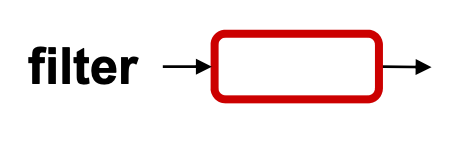
\includegraphics[width=0.5\textwidth]{figures/StreamItFilter.png}
  \centering
  \caption{StreamIt Filter}
  \label{fig:filter}
\end{figure}

\paragraph{Pipeline}
High level abstraction of a software pipeline among filters.

Allow the programmer to specify a set of filters that are connected through a pipeline connection; this allow the compiler to exploit pipeline parallelism.

\begin{figure}[h!]
  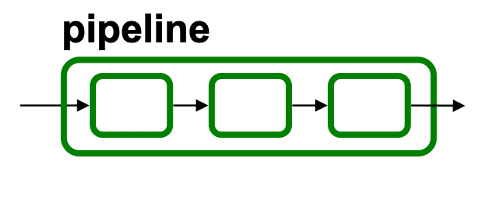
\includegraphics[width=0.5\textwidth]{figures/StreamItPipeline.png}
  \centering
  \caption{StreamIt Pipeline}
  \label{fig:pipeline}
\end{figure}

\paragraph{SplitJoin}
Allow the specification of multiple parallel and independent computation paths that diverge from a common splitter and merge into a common joiner.

Can be used to extract both task level and data level parallelism. 
If all items are sent to all filters and and each filter perform a different transformation on the data item it extract task level parallelism; if the incoming data stream is load balanced among the different filters and all filters perform the same operation it extract data level parallelism. The behavior of the SplitJoin construct is thus defined by the behavior of the splitter and the joiner blocks.

\begin{figure}[h!]
  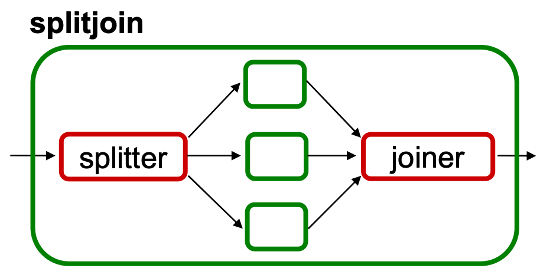
\includegraphics[width=0.5\textwidth]{figures/StreamItSplitJoin.png}
  \centering
  \caption{StreamIt SplitJoin}
  \label{fig:splitjoin}
\end{figure}

\paragraph{Feedback loop}
Allow the creation of loops in the computation.

Wrap a main body filter in a feedback loop; the data items that enter the section are merged with the feedback connection through a joiner block while the items that exit the body filter are splitted between the feedback connection and the next filter according to a splitter block. 

The programmer can also define a computation path along the feedback connection, this allow transformations on items that are sent along the feedback connection.

\begin{figure}[h!]
  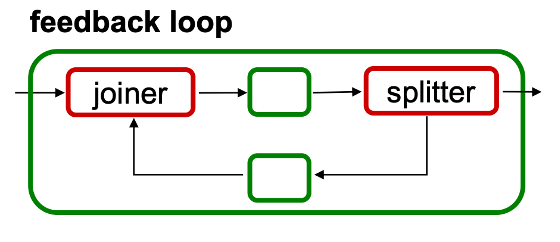
\includegraphics[width=0.5\textwidth]{figures/StreamItFeedbackLoop.png}
  \centering
  \caption{StreamIt Feedback Loop}
  \label{fig:feedback}
\end{figure}

\subsection{Compilation Infrastructure}
The StreamIt compilation infrastructure is designed to start from the high level abstraction of a StreamIt program and produce the final application to be deployed. 
The programmer describe the application in terms of which transformations need to be applied to each item and how different transformations are connected; then, the StreamIt compiler automatically optimize the StreamIt program for the streaming context and produce the final optimized code for the target back end.

\subsubsection{Stream Graph Scheduling}
One of the most important pieces of information that is compiled from the StreamIt code is the Stream Graph of the application. The Stream graph is an internal representation of the streaming application that represent how different actors interact; the StreamIt compiler use it to retain information about how different filters interact and the amount of parallelism that can be exploited among filters.

The goal of the Stream Graph Scheduling phase is to find a steady state schedule that allow the program to process the stream of input items while maintaining constant the number of live items on each communication channel.

\subsubsection{Partitioning}
Given the Stream Graph and the steady state schedule of the application the compiler need to adapt the computation to the granularity of the target architecture. 
The Stream Graph compiled from the StreamIt program do not take into consideration the number of processing elements. Mapping directly the original nodes to physical processors would lead to unoptimized results; in case of a too coarse grained graph the program would not use some processing elements, in case of a too fine grained graph the final program would require unnecessary memory communication.
The Streamit compiler use a heuristic to decide the number of nodes to be mapped to physical elements, the graph is adapted by producing a new graph with a number of nodes that match the number of processing elements of the target architecture.
In order to create the new stream graph, the compiler must implement Fusion and Fission operations. Fusion merge two filters into one and Fission does the opposite operation. Fusion and Fission are not simple operations, the compiler must take into consideration the type of connections between filters in order to apply these operations efficiently.

To partition the stream graph in a set of balanced filters, the compiler must be able to estimate the amount of work performed by the work function of each filter. StreamIt estimate the work through static inspection. Since the number of iterations of each loop is known at compile time, the compiler can estimate the total amount of work by unrolling each loop and considering the number and the type of instructions executed at each fire. 

The partitioning phase can then be performed automatically with a simple greedy algorithm that split the most demanding filters and merge the least demanding ones.

\subsubsection{Layout}
Given the work balanced nodes from the partitioning phase, the StreamIt compiler need to assign each node to a physical node on the target architecture while minimizing the communication overhead between nodes.
To optimize the communication and synchronization overhead a back end dependent cost function must be defined and optimized. The Cost function should accurately measure the added communication and synchronization generated by mapping the work balanced Stream Graph to the communication model of the target. 


\subsubsection{Communication scheduler}
When the layout phase has mapped filters to physical computation nodes the only remaining abstraction that need to be mapped to the target architecture is the communication queues between filters. The communication scheduler maps the infinite FIFO abstraction to the limited resources of the target architecture while avoiding deadlocks and starvation.

Once the Communication Scheduler phase is finished the StreamIt compiler is ready to generate the final code for the target back-end.

\section{VitisAI}
\label{vitis}

VitisAI is a development stack for AI inference on Xilinx's HW; it is a complete development stack to optimize and deploy a pretrained model on FPGA without the need of knowing any implementation detail about the underlying HW.

\begin{figure}[h!]
  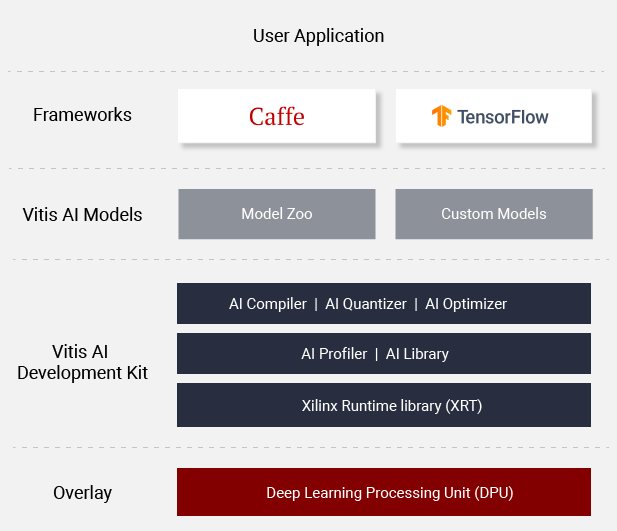
\includegraphics[width=0.5\textwidth]{figures/Vitis-AI-Stack.png}
  \centering
  \caption{Vitis AI stack}
  \label{fig:VitisAIStack}
\end{figure}

The programmer can feed to the VitisAI stack an abstract model in ONNX format or defined with one of the most common frameworks. The stack automatically optimize the model for the target architecture with few optimization tools and produce the final program to be deployed on the target Xilinx architecture.

\subsection{Optimization tools}
The stack have multiple free tools that can be used to perform optimizations on the input model; these optimization tools can also be used as preprocessing steps on an abstract model before feeding it to a different stack.

\paragraph{AIOptimizer}
Perform pruning on the input model, it automatically prune the connections between artificial neurons that less affect the accuracy of the final model.

\paragraph{AIQuantizer}
Automatically convert the floating-point precision of the input model's weights to a fixed-point representation. This is especially useful on FPGA since it is possible to use a completely custom number of bits without being restricted by the HW design.

\paragraph{AICompiler}
The quantizer perform HW depentant optimizations on the quantized model, it maps the model to optimized DPU instructions while performing optimizations like node partitioning and instruction scheduling.

\section{Halide}
\label {halide}
With the increasing size of deep learning models and the widening gap between processing power and memory bandwidth it is increasingly difficult to train and deploy new and more computationally demanding DL models. A possible solution might be to write custom code to exploit the right trade-off among data locality, recomputation and parallelism but the process is slow, prone to errors, do not allow for fast prototyping of different scheduling solutions and the programmer has a constant focus on implementation details. 
Halide is a language and compiler to write high performance tensor processing pipelines for multiple target platforms with the goal of solving the emerging problems of image processing pipelines and deep learning applications; the Halide domain-specific language allow to separately define the algorithm that need to be executed, as functions of the input tensor, and the scheduling strategy to be applied for the specific algorithm on the target architecture. Decoupling the definition of a Halide program in two different components allow the exploration of a large number of scheduling strategies with far fewer lines of code and without affecting the correctness of the program.

\subsection{Algorithm definition}
The Halide algorithm describe what the programmer want to compute without defining how the final result should be computed; this guarantee the correctness of the final program while experimenting with different scheduling strategies and leave to the compiler the responsibility of optimizing the final code.
The Halide DSL represent the algorithm definition as an Abstract Syntax Tree of 3 main components: Variables, expressions and functions.

Each function is defined over a set of variables and it's value is computed as an expression of other functions. As example we can use the 3x3 blur filter definition:

\[ \mathsf{blur\_x}(x, y) = (\mathsf{input}(x-1, y) + \mathsf{input}(x, y) + \mathsf{input}(x+1, y))/3;\]
\[ \mathsf{blur\_y}(x, y) = (\mathsf{blur\_x}(x, y-1) + \mathsf{blur\_x}(x, y) + \mathsf{blur\_x}(x, y+1))/3;\]

The pipeline is composed by 2 functions, blur\_x and blur\_y; both functions are defined over two different dimensions that define the x and y coordinates of the image. The value of each function is an expression composed as the mean of the 3 nearest pixels in both directions.


\subsection{Schedule definition}
Now that the algorithm is defined Halide need to know how to compute the results in terms of storage and compute granularity. Storage granularity and compute granularity refer to how big the buffers between stages need to be and how frequently consumers and producers are interleaved.

One possible naive solution might be to compute and store each stage of the pipeline one at a time and separately from from others; this is actually the approach of the most common frameworks, after each stage the results are stored in main memory before proceeding with the next stage of the pipeline. This approach suffer of the drawback of having poor locality since every tensor must be computed and stored in its entirety and is unlikely to fit into a low level memory. 
A second possible approach is to compute only the last stage of the pipeline without storing intermediate results; this maximize locality by recomputing every value each time but require an amount of work that grow exponentially with the number of stages in the pipeline.
A third approach is to allocate large buffers while performing fine-grained computation, this allow for solving both problems by reusing all previously computed results while exploiting locality. The problem of this last approach is the introduction of dependencies into computed results thus reducing the amount of parallelism that can be exploited from different chunks of work.
The programmer should find the right trade-off by using store\_at and compute\_at directives and by performing tiling, unrolling and reordering operations on different pipeline stages.

An other important decision to be made by the schedule is how to use HW specific features to increase the pipeline performances (such as multiple cores, vectorized instructions, GPUs, and so on..). The schedule allow the programmer to combine in different ways different features for each variable and function; this make easier for the programmer to explore different acceleration strategies without touching the code that defines the algorithm.

Finding the right schedule to manage storage and compute granularity while exploiting the HW specific features is not a trivial task, especially when considering complex pipelines for complex image filters and DL applications. For that reason Halide have a built in autoscheduler to automatically find a schedule; the current version require extensive optimization to find a schedule that is as good as one manually created by a expert programmer and can be used to find a baseline in a small amount of time.

To make an example we can take again the 3x3 blur filter:

\[ \mathsf{blur\_y.tile}(x, y, xi, yi, 256, 32)\mathsf{.vectorize}(xi, 8)\mathsf{.parallel}(y);\]
\[ \mathsf{blur\_x.compute\_at}(blur\_y, x)\mathsf{.vectorize}(x, 8);\]

The schedule use both parallelization and vectorization operations, tile the loop nest and compute blur\_x for each unique value of the variable x of blur\_y. The programmer only need to specify how the computation is performed, Halide takes case of all implementation details and generate efficient code.

\subsection{Halide Compiler}

The Halide compiler take as input both the algorithm definition and the schedule and produce a cross platform internal representation. The internal representation is then optimized by performing target independent optimizations and compiled into the final code of the target back-end.

\begin{figure}[h!]
  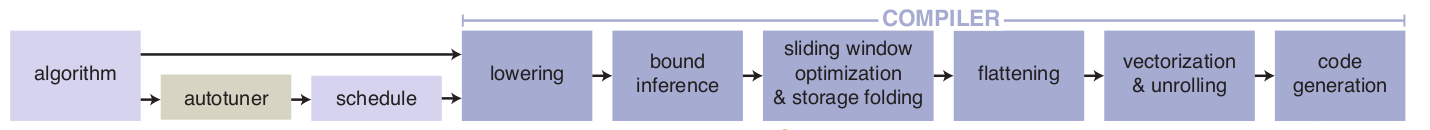
\includegraphics[width=1\textwidth]{figures/HalideCompilerStack.png}
  \centering
  \caption{Halide stack}
  \label{fig:HalideStack}
\end{figure}

The first step ot the Halide compilation infrastructure is to lower the algorithm and schedule definition to a set of loop nests and buffer allocations. Each loop is labeled as serial, parallel, unrolled or vectorized and loop bounds are left as symbolic expressions of the required region of the output function.
The lowering process start from the output function and recursively proceeds backward toward input functions. 
The process is complete once all functions has been lowered.

Once the Lowering process has been completed the Halide compiler stack have a complete representation of the Halide program as a loop nest operating on multidimensional tensor objects. The compiler know the set of loops and the number of dimensions that are required to compute the final result but do not know the extend of such dimensions.
The Bound Inference procedure is a two step process. The first step calculate the extends of each tensor; the compiler propagate backward the information about the size of the output tensor and calculate recursively the extents of intermediate bounds. The second step use this information to calculate the extent of each loop.

By knowing the extend of each dimension, Halide can traverse the loop nest to seek for sliding window and storage folding optimizations. These two optimizations passes are used to leverage the storage granularity allowed in the current schedule and reuse data already computed in previous iterations.

The optimized sequence of loop nests with multi-dimensional store and load is then lowered to a single-dimensional strided representation. Each multi-dimensional tensor is converted into a single-dimensional representation and each load and store operation on tensor is represented as a stride access on the corresponding single-dimensional buffer.

The final step before invoking the target back-end to compile the Halide IR into the final code is to remove unrolled and vectorized loops. 
Unrolled loops can be simplified by performing the loop unrolling operation directly on the halide IR while vectorized loops can be removed by replacing them with dense memory accesses and operations using ramps to represent strided sets of indexes on memory buffers.

\subsection{Deep learning applications}
DL models are composed by a sequence of layers that can be expressed as an Halide algorithm by composing functions and expressions. As for other most common DL frameworks Halide automatically differentiate feed forward models; the programmer only need to define the model structure and the Automatic Differentiation return a new function that calculate the requested derivatives.
The Halide Automatic Differentiation system must take into consideration some optimizations to exploit as much parallelism as possible while performing gradient propagation on scatter-gather operations; since gather operations become become scatter operations  when differentiated and scatter operations are not easily parallelizable, the Automatic Differentiation system automatically convert scatter operations back to gather operations to allow a higher degree of exploitable parallelism in the final gradient function.

Since the increasing complexity of modern DL models are making impractical the definition by hand of a model as an Halide algorithm the programmer can provide an abstract definition with a cross-platform format like ONNX. Providing an abstract model avoid to the programmer the tedious and error prone work of defining a model as composition of functions. Halide automatically convert the ONNX model to an Halide algorithm and return a function that can be used to perform inference or differentiated through automatic differentiation to calculate the gradient for the backpropagation algorithm.


\chapter{From ONNX model to Bambu HLS}
In this chapter we introduce the main contribution of this thesis, we describe the proposed design flow and how it is implemented as part of the Halide infrastructure. 
In section \ref{motivations} we describe the motivations to use HLS tools to deploy DL models on FPGAs. We describe the main HW platform that can be used to perform inference and their drawbacks. 
In section \ref{back-end} we describe how the Bambu back-end works and how it is implemented inside the Halide infrastructure. We describe the main steps and possible future improvements.
\newpage

\section{Motivations}
\label {motivations}
Since the state of the art DL models are becoming increasingly more complex and demanding in terms of computational power, using CPUs and GPGPUs as inference platforms is becoming a less appealing approach. 
When a model is deployed the system is required to satisfy latency, throughput and memory consumption constraints; CPUs are not suitable for high throughput applications and power hungry GPUs have high latency due to memory transfers between host and accelerator.
The use specialized ASICs meet all 3 requirements with high throughput, low latency and memory consumption; but such a solution is not flexible and not able to express new layers that might have not been yet invented.

A different approach is to use Field Programmable Gate Arrays (FPGA); the use of programmable HW allow the possibility to satisfy all system requirements while being able to use the system to deploy different models.
The problem with FPGAs is the time required to deploy an FPGA's application; deploying a correct and optimized bitstream is not trivial and require a long design time. To reduce that problem High Level Synthesis tools are used; these tools take as input the abstract representation of a program, in this case a DL models, and produce as output the optimized bitstream to be deployed. The final result do not have the same performance that a manually designed and optimized solution would have but allow fast prototyping and the use of FPGAs to deploy models without the need of being an expert of the design process.

The integration of a Bambu back-end in Halide allow the programmer to easily deploy a DL model on FPGA; the decoupling of the schedule from the algorithm definition allow the programmer to leverage the possibility to deploy multiple models in a short amount of time and find the schedule that better fit the target architecture and memory hierarchy.

\section{Design flow}
\label {design-flow}
The goal of the proposed design flow is to leverage PandA - bambu and the Halide infrastructure to deploy a Deep Learning model on FPGA while being able to optimize the sequence of scheduled operations for the target architecture.

\begin{figure}[h!]
  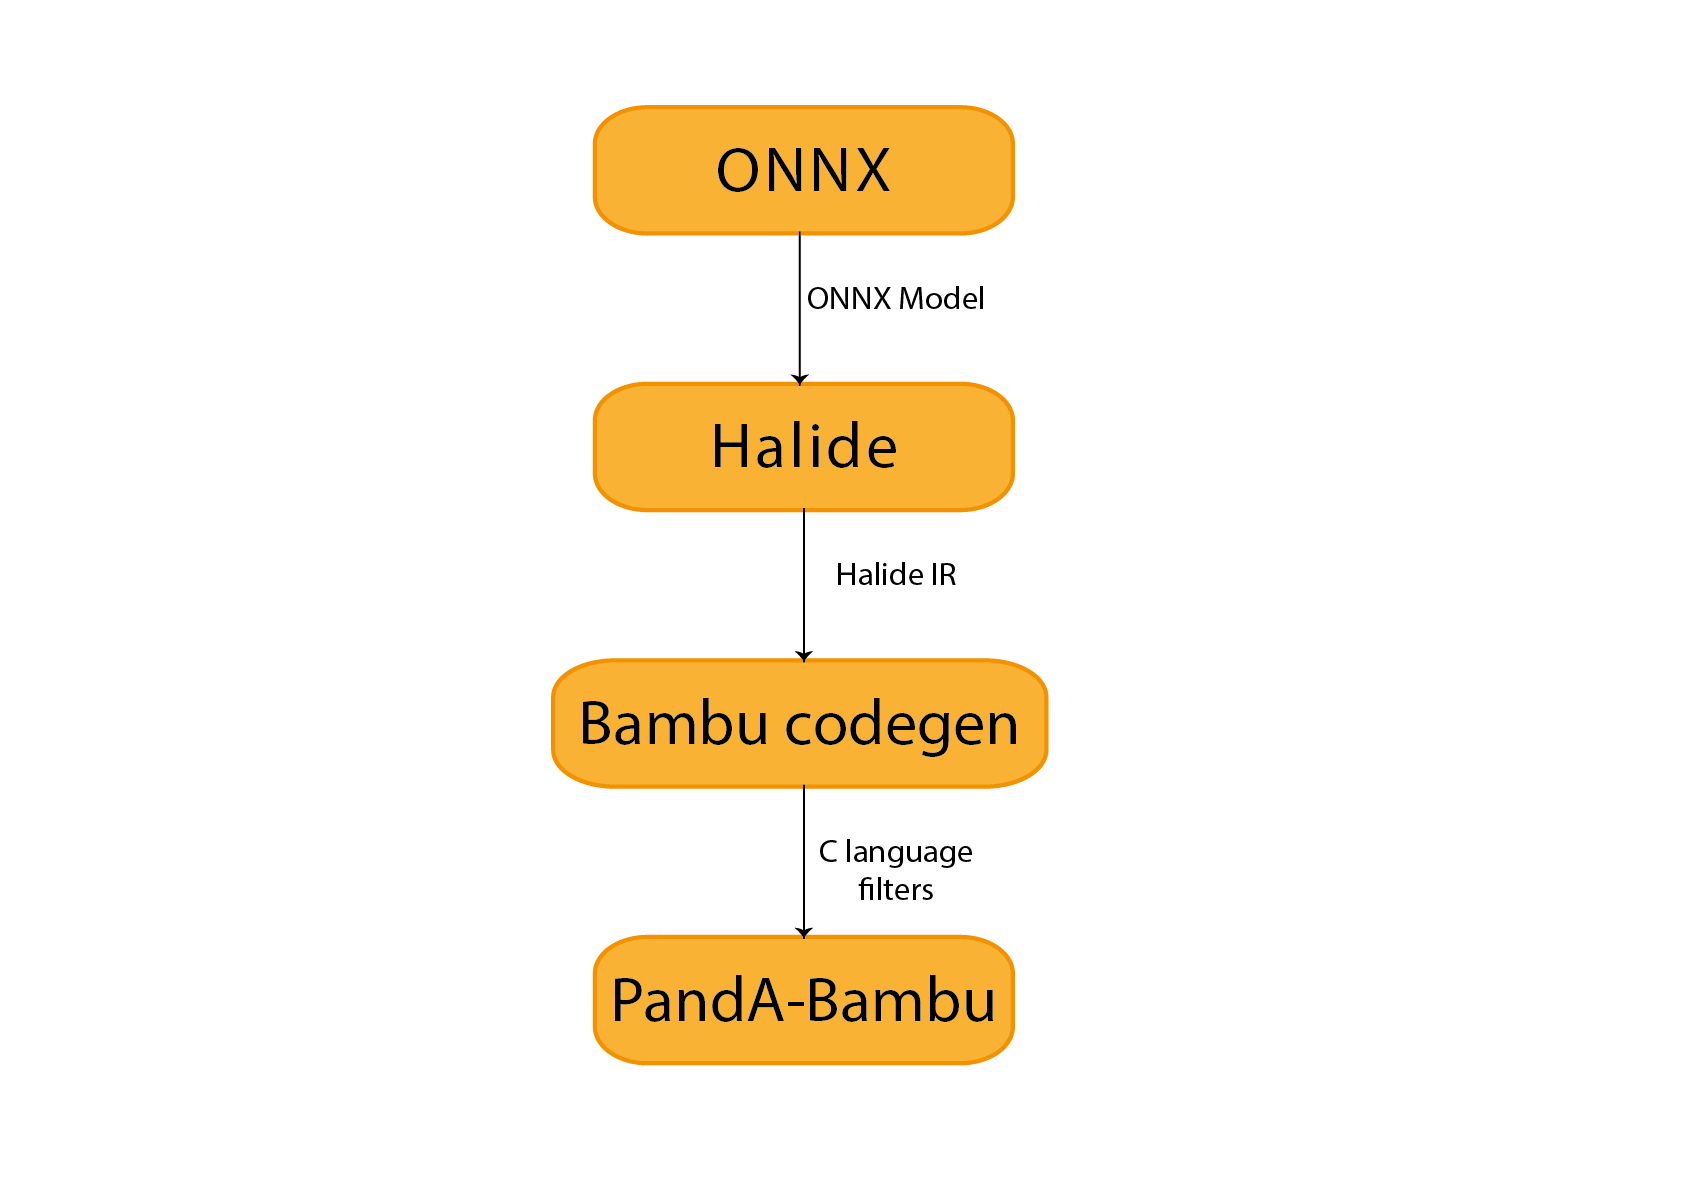
\includegraphics[width=1\textwidth]{figures/Stack.png}
  \centering
  \caption{Design Flow}
  \label{fig:DesignFlowStack}
\end{figure}

The starting point is a Deep Neural Network model provided from one of the most common frameworks. Since each framework represent the computational graph in different ways we to use a common representation to provide a unique entry point to the proposed design flow. The Open Neural Network eXchange specification (ONNX) has been used as common representation; using ONNX allows the portability of computational graphs between different frameworks and is already supported by the Halide infrastructure.

To increase the performance of a forward pass of a DL models the design flow incorporate two optional steps: By using the VitisAI tools the programmer can perform pruning and quantization on the ONNX model. The pruning optimization increase the performance of the final model by reducing the amount of work that has to be done by removing the less useful connections between neurons and the quantization reduce the floating point precision of the operations. The latter is especially useful for FPGAs since the floating point precision can be easily adapted. 

Given the ONNX model that need to be deployed the Halide framework have a built-in tool to convert it to a internal generator. The programmer can then decide how to schedule the imported model by defining the schedule method of the generator, as for any other algorithm. 

Halide can then proceed by converting the scheduled generator to a internal IR before feeding the optimized representation to the Bambu back-end that has been developed to provide support for FPGA targets.


\section{The Bambu back-end}
\label {back-end}
To implement a new back-end the Halide infrastructure allow the creation of target specific codegens that take as input the Halide IR and produce the final optimized code. Each target architecture have it's own back-end, that allow the Halide infrastructure to take advantage of architecture specific features and optimizations.

The Bambu back-end take as input the Halide IR and produce the C code to be used within the bambu framework. The code generation is split in 3 main steps: Filters extraction, IR optimizations and code generation. In the next sections describe the three steps in details.

\subsection{Filters extraction}
The filters extraction step take as input the Halide IR and produce a DAG representation of the Halide lowered function. 
The DAG is composed by interconnected filters related by a producer consumer relationship. 
Such relationship is already extracted by the Halide infrastructure and can be easily extracted by leveraging the ProducerConsumer statement of the Halide IR.

\begin{lstlisting}[caption= Example of filter extracted from the Halide IR. The extracted code is hard to translate to c language and access the memory buffers at each iteration. ]
X_im_padded_U_sum_3[0] = 0.000000f
for (x_7, 0, 3) {
    for (x_8, 0, 3) {
        X_im_padded_U_sum_3[0] = ((float32)X_im_padded_U_sum_3[0] 
          + ((float32)b2[((x_7*6) x_3)]
          * ((float32)b2[((x_8*6) + x_4)]
          * (float32)b0[((((x_2*3) + x_8)*3) + x_7)])))
    }
}
\end{lstlisting}

Before proceding with the extraction of the DAG filters the codegen clean the IR representation by removing unused constructs, renaming variables and buffers to avoid name conflicts and by substituting into the IR values that are already known at compile time such as the dimensions of the input and output tensors. 
This improves the bound inference analysis of the Halide compiler by reducing the number of variables and increasing the number of fixed size loops inside the Halide IR. 

Once the IR has been preprocessed the producer consumer filters can be extracted.
Each filter of the DAG representation is going to be fully described by the IR code of the filter and the connections with other filters.
Other information about buffers and variables usage are stored in order to make easier the work of subsequent steps.

When the schedule store multiple functions at root granularity the resulting DAG have multiple filters without incoming dependencies. 
This introduce a entry point problem when trying to generate the final code. 
To solve such problem a new base filter is always introduced; the bambu\_main\_filter work as entry point for the computation and is used to store the necessary buffers and call the filters with root store granularity.

\subsection{IR optimizations}
Once the filters has been extracted the program has been represented as a set of interconnected independent filters related by producer consumer relationships. Each filter have its own independent code represented as a Halide statement. The IR code of each filter can be optimized by performing a set of basic optimization passes over the IR code representation such as reducing as much as possible redundant memory accesses and by avoiding recomputation of data shared by different iterations.

The first operation that is performed is the IR preparation for subsequent optimization passes. Each IR operation is split into multiple statements that perform basic operations such as single operators and call to external functions.
Such operation also improve the readability of the generated code.

The first optimization pass performed is pushing each store as outside as possible of the loop nest. This is performed by computing for each store the dependency on other variables and by pushing an operation outside a for loop only if the operation do not depend on the variable of the loop. This allow the final code to avoid recomputation of data shared among different iterations inside the filter execution.
The second optimization pass performed is the fix of multiple read writes on the same buffer inside the filter code. The Halide IR represent the computation by operating directly on the buffer memory. This is not an optimized approach for the code to be generated. When a filter code access a buffer location on the same index inside the same loop the IR is optimized by pushing as outside as possible the read and write memory access inside the IR. The previous memory operations are replaced with access to local variables. 

\begin{lstlisting}[caption = Example of optimized IR. The complex operation of the previous example has been split into simple operations. Intermediate results that are shared among different iterations and memory accesses has been pushed outside]
X_im_padded_U_sum_3[0] = 0.000000f
_9[0] = (x_2*3)
_17[0] = (float32)X_im_padded_U_sum_3[0]
for (x_7, 0, 3) {
    _3[0] = (x_7*6)
    _4[0] = (_3 + x_3)
    for (x_8, 0, 3) {
        _6[0] = (x_8*6)
        _7[0] = (_6 + x_4)
        _10[0] = (_9 + x_8)
        _11[0] = (_10*3)
        _12[0] = (_11 + x_7)
        _2[0] = (float32)_17
        _5[0] = (float32)b2[_4]
        _8[0] = (float32)b2[_7]
        _13[0] = (float32)b0[_12]
        _14[0] = ((float32)_8*(float32)_13)
        _15[0] = ((float32)_5*(float32)_14)
        _16[0] = ((float32)_2 + (float32)_15)
        _17[0] = (float32)_16
    }
}
\end{lstlisting}
A third optimization pass is the elimination of trivial buffers of size of one element. When a filter operate on a buffer of single size the buffer is replaced with a variable and is passed to the called filter as a single variable. When the buffer with a size of one element is instead the output buffer the filter return the computed value as the return value of the function representing the filter execution.

An other important optimization is the detection of situations when producer consumer operations allow the usage of FIFO queues to send data between filters. 
If such a situation holds, the memory access on a buffer can be replaced with a FIFO queue. 
FIFO queues are already implemented and optimized inside the Bambu framework; using such a communication channel can improve the memory management of processed values among filters.
At the moment FIFO queues are detected in the trivial case of single read and write accesses on matching indexes and loop nests. 
A future work might improve the detection of FIFO channel by detecting sliding window optimizations 

Once the IR optimization passes has been performed on all filters the DAG is ready to be translated into the C function to be feed to the Bambu framework.

\subsection{Code generation}
After the optimization step the codegen is ready to produce the final code to be used with the Bambu framework. The work is carried out by simply visiting the IR and translating line by line the IR operations to corresponding C operations. To avoid loss of floating point precision when writing constants we decided to write the value of each constant as hexfloat values.

\begin{lstlisting}[caption = Output C code of the example filter. The Halide IR has been translated to C code and encapsulated. Since the filter compute only one value a return statement has been added at the end of the function.]
float X_im_padded_U_sum_3_fun_0(float b0[18], float b2[18],
        int x_2, int x_3, int x_4){
    float X_im_padded_U_sum_3 = 0x0p+0;
    X_im_padded_U_sum_3 = 0x0p+0;
    int32_t _9 = x_2 * 3;
    float _17 = X_im_padded_U_sum_3;
    for(unsigned int x_7 = (0); x_7 < (0 + 3); x_7++){
        int32_t _3 = x_7 * 6;
        int32_t _4 = _3 + x_3;
        for(unsigned int x_8 = (0); x_8 < (0 + 3); x_8++){
            int32_t _6 = x_8 * 6;
            int32_t _7 = _6 + x_4;
            int32_t _10 = _9 + x_8;
            int32_t _11 = _10 * 3;
            int32_t _12 = _11 + x_7;
            float _2 = _17;
            float _5 = b2[_4];
            float _8 = b2[_7];
            float _13 = b0[_12];
            float _14 = _8 * _13;
            float _15 = _5 * _14;
            float _16 = _2 + _15;
            _17 = _16;
        }
    }
    X_im_padded_U_sum_3 = _17;
    return X_im_padded_U_sum_3;
}
\end{lstlisting}

The result is the set of final filters written in C language and ready to be deployed.

\section{Conclusions}
In this section we described the structure of the design flow. We described the steps necessary to optimize and deploy a DL models using the ONNX representation, the Halide infrastructure and PandA-Bambu as HLS tool. We described how is the Halide Bambu codegen structured and how it work.



\backmatter

\listoffigures
\addcontentsline{toc}{chapter}{\listfigurename}

\listoftables
\addcontentsline{toc}{chapter}{\listtablename}


%%% create index %%%
\printindex

\begin{thebibliography}{9}
\addcontentsline{toc}{chapter}{Bibliography}

%\bibitem{latexcompanion} 
%Michel Goossens, Frank Mittelbach, and Alexander Samarin. 
%\textit{The \LaTeX\ Companion}. 
%Addison-Wesley, Reading, Massachusetts, 1993.
 
 
\end{thebibliography}

\end{document}

